%% 
%% Copyright 2007, 2008, 2009 Elsevier Ltd
%% 
%% This file is part of the 'Elsarticle Bundle'.
%% ---------------------------------------------
%% 
%% It may be distributed under the conditions of the LaTeX Project Public
%% License, either version 1.2 of this license or (at your option) any
%% later version.  The latest version of this license is in
%%    http://www.latex-project.org/lppl.txt
%% and version 1.2 or later is part of all distributions of LaTeX
%% version 1999/12/01 or later.
%% 
%% The list of all files belonging to the 'Elsarticle Bundle' is
%% given in the file `manifest.txt'.
%% 
%% Template article for Elsevier's document class `elsarticle'
%% with harvard style bibliographic references
%% SP 2008/03/01

%\documentclass[preprint,12pt,authoryear]{elsarticle}  %default in the template
%\documentclass[preprint,10pt,authoryear]{elsarticle}

%% Use the option review to obtain double line spacing
%% \documentclass[authoryear,preprint,review,12pt]{elsarticle}

%% Use the options 1p,twocolumn; 3p; 3p,twocolumn; 5p; or 5p,twocolumn
%% for a journal layout:
%% \documentclass[final,1p,times,authoryear]{elsarticle}
%% \documentclass[final,1p,times,twocolumn,authoryear]{elsarticle}
 \documentclass[final,3p,times,authoryear]{elsarticle}
%% \documentclass[final,3p,times,twocolumn,authoryear]{elsarticle}
%% \documentclass[final,5p,times,authoryear]{elsarticle}
%% \documentclass[final,5p,times,twocolumn,authoryear]{elsarticle}

%% For including figures, graphicx.sty has been loaded in
%% elsarticle.cls. If you prefer to use the old commands
%% please give \usepackage{epsfig}

%% The amssymb package provides various useful mathematical symbols
\usepackage{amssymb}
%% The amsthm package provides extended theorem environments
\usepackage{amsthm}
\usepackage{amsmath}
\usepackage{color, colortbl}
\usepackage{amsmath}
\usepackage{siunitx}
%\usepackage{todonotes}
\usepackage{tabularx}
\usepackage[]{algorithm2e}
\usepackage{soul}
%\usepackage[colorinlistoftodos]{todonotes}

\usepackage{xargs}
\usepackage[pdftex,dvipsnames]{xcolor}
\usepackage[colorinlistoftodos,prependcaption,textsize=tiny]{todonotes}
\newcommandx{\unsure}[2][1=]{\todo[linecolor=red,backgroundcolor=red!25,bordercolor=red,#1]{#2}}
\newcommandx{\change}[2][1=]{\todo[linecolor=blue,backgroundcolor=blue!25,bordercolor=blue,#1]{#2}}
\newcommandx{\info}[2][1=]{\todo[linecolor=OliveGreen,backgroundcolor=OliveGreen!25,bordercolor=OliveGreen,#1]{#2}}
\newcommandx{\improvement}[2][1=]{\todo[linecolor=Plum,backgroundcolor=Plum!25,bordercolor=Plum,#1]{#2}}
\newcommandx{\thiswillnotshow}[2][1=]{\todo[disable,#1]{#2}}

\definecolor{light-gray}{gray}{0.9}

\usepackage{framed} % Framing content

\DeclareRobustCommand{\hlgreen}[1]{{\sethlcolor{green}\hl{#1}}}

\journal{Urban Climate}



\begin{document}

%\runninghead{Nice et al.}

\title{COVID-19 lockdowns: The impact on pollution, mobility, and energy use.}

\author[melb]{Kerry~A.~Nice\corref{cor1}\fnref{label1}}
\author[melb]{Jasper S. Wijnands\fnref{label1}}
%\author[melb]{Jason Thompson}
%\author[melb]{Sachith Seneviratne}
%\author[melb]{Haifeng Zhao}
%\author[melb,eng]{Mark Stevenson}
\cortext[cor1]{Principal corresponding author}
\address[melb]{Transport, Health, and Urban Design Hub, Faculty of Architecture, Building, and Planning, University of Melbourne, Australia.}
%\address[eng]{Melbourne School of Engineering; and Melbourne School of Population and Global Health, University of Melbourne, Australia.}
\fntext[label1]{These authors contributed equally to this work}






\begin{abstract}

\end{abstract}

\begin{keyword}
COVID-19\sep 
pollution\sep
city science
\end{keyword}



\maketitle

\section{Methods}
\subsection{Data sources}

\subsubsection{Pollution data}
The World Air Quality Index project \citep{AQICN2021} provides ground-level readings of pollutants for about 2000 cities in 132 countries sourced from world-wide environmental protection agencies. We downloaded data for about 900 cities for 2014-2021. The pollutants downloaded were PM$_{2.5}$, PM$_{10}$, O$_{3}$, NO$_{2}$, SO$_{2}$ and CO. AQICN converts all readings from mg/m$^{3}$ to AQI levels using the EPA standard and provides a 24 hour average of hourly readings.

(of the 1672 largest cities in the world\citep{UNDESA2015})

Air Quality Index scale as defined by the US-EPA 2016 standard

\subsubsection{Stringency index}

Oxford Covid-19 Government Response Tracker \citep{Hale2020} (Figure \ref{fig:oxcgrt}) daily stringency index is based on a combination of containment and closure policies and assigned an ordinal value (0 to 1, 2, 3, or 4 depending on the indicator). These include school closings, workplace closings, cancellation of public events, restrictions on gatherings, closing public transport, stay at home requirements, restrictions on internal movements, international travel controls and government public information campaigns. These are combined into an index and scaled 0-100. Each of the containment policies are also available individually. In addition, indexes are available at a state (and selected city) level for the United States and Brazil \citep{Hale2020a,Petherick2020} (Figure \ref{fig:statestr}).




\begin{figure*}
\centering
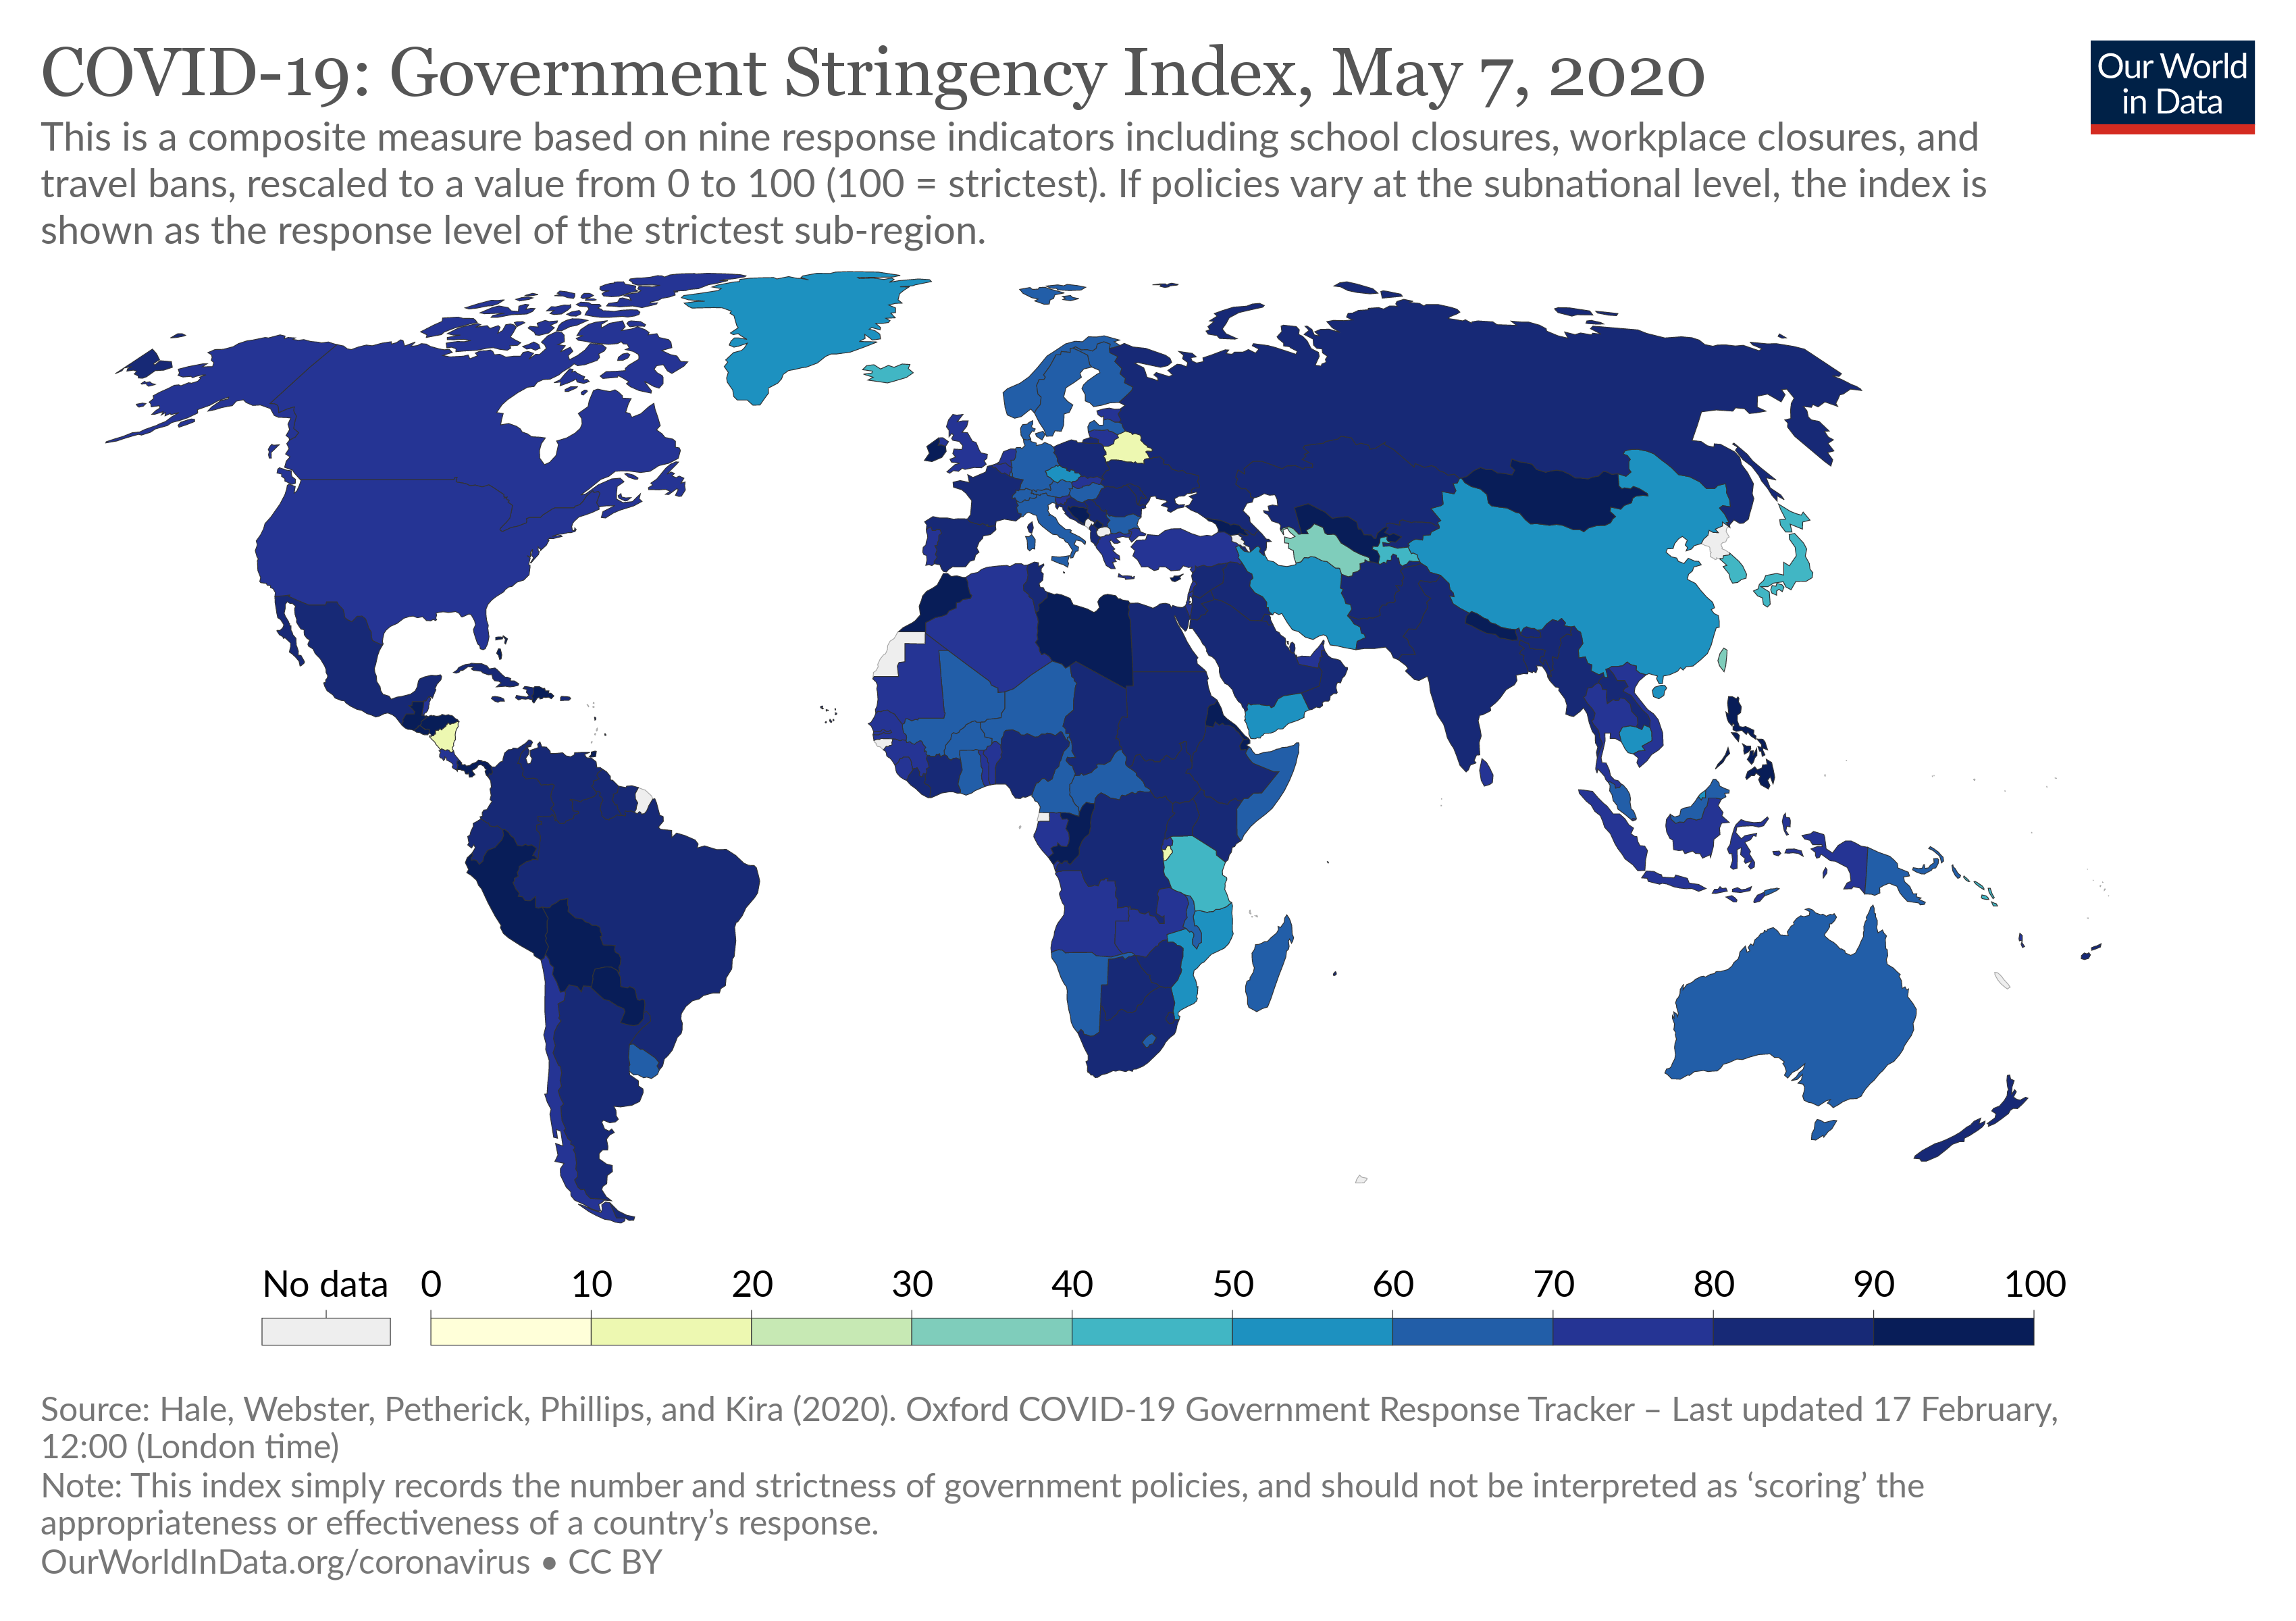
\includegraphics[width=.99\linewidth]{images/covid-stringency-index.png}
\caption{Oxford Covid-19 Government Response Tracker daily stringency index.}
 \label{fig:oxcgrt}
\end{figure*} 

\begin{figure*}
\centering
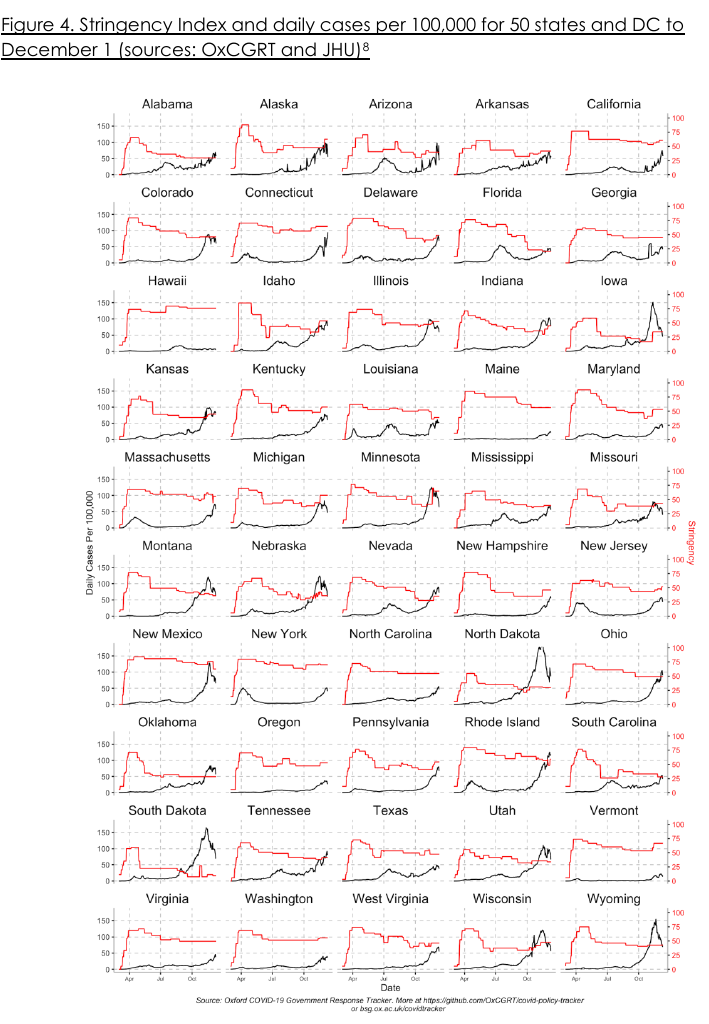
\includegraphics[width=.99\linewidth]{images/Hallas2020-stateStr.png}
\caption{Stringency index and daily cases per 100,000 for 50 states and DC to December 1\citep{Hallas2020}.}
 \label{fig:statestr}
\end{figure*}


\subsubsection{Mobility data}
\paragraph{Google}

Google COVID-19 Community Mobility Reports \citep{Google2020} provides a  daily percentage change of visitors to retail and recreation, grocery and pharmacy, parks, transit stations, workplaces, and residences from a historic baseline. The baseline is a median value from January 3 to February 6, 2020. This data is at a county/province level for all data. We mapped this data to the cities included in these or by combining multiple counties into a single city. Figure \ref{fig:googlemobility} shows mobility trends for Melbourne, Australia across 2020 and 2021.

\begin{figure*}
\centering
\includegraphics[width=.99\linewidth]{images/{"city90_Melbourne, Australia"}.png}
\caption{Google mobility data for Melbourne, Australia across 2020 and 2021.}
 \label{fig:googlemobility}
\end{figure*}


\paragraph{Apple}
Apple Maps Mobility Trends Reports \citep{Apple2020} provides a daily percent change in Apple Maps routing requests from the baseline January 13, 2020 for driving, walking, and public transport journeys. This data is at a county/province level for all data. We mapped this data to the cities included in these or by combining multiple counties into a single city. Figure \ref{fig:statestr} shows mobility trends for Melbourne, Australia across 2020 and 2021.

\paragraph{Apple}
\begin{figure*}
\centering
\includegraphics[width=.99\linewidth]{images/{"Apple_city90_Melbourne, Australia"}.png}
\caption{Apple Maps mobility data for Melbourne, Australia across 2020 and 2021.}
 \label{fig:statestr}
\end{figure*}

\subsubsection{Monthly electricity statistics}
The International Energy Agency produces reports of electricity generation and usage for 47 countries for 2016-2020 \citep{IEA2021}. These reports break down monthly generation through conventional thermal and combustibles (coal, oil, natural gas, and others) and renewables (nuclear, hydro, wind, solar, and geothermal). These reports are at a country level. We mapped the country level data to each individual city. Figure \ref{fig:au-total} shows trends of Australian net electricity production from all sources 2016-2021 and trends of conventional thermal (Figure \ref{fig:au-thermal}) over the same period. Figure \ref{fig:china-net} shows Chinese electricity generation through coal 2016-2021.

\subsubsection{Energy usage}
\paragraph{Apple}
\begin{figure*}
\centering
\includegraphics[width=.99\linewidth]{images/{"AUSTRALIA_TOTAL NET PRODUCTION"}.png}
\caption{Trends of Australian net electricity production from all sources 2016-2021.}
 \label{fig:au-total}
\end{figure*}

\begin{figure*}
\centering
\includegraphics[width=.99\linewidth]{images/{"AUSTRALIA_CONVENTIONAL THERMAL"}.png}
\caption{Trends of Australian electricity production from conventional thermal 2016-2021.}
 \label{fig:au-thermal}
\end{figure*}

\begin{figure*}
\centering
\includegraphics[width=.99\linewidth]{images/{"CHINA_TOTAL NET PRODUCTION"}.png}
\caption{Trends of Chinese electricity production from coal 2016-2021.}
 \label{fig:china-net}
\end{figure*}


\section*{References}\label{sec:ref}

  \bibliographystyle{elsarticle-harv} 
 % \bibliography{bib}
   \bibliography{COVID.bib}


\end{document}
